  
\documentclass{beamer}
\usepackage{listings}
\usepackage{graphicx}
\usepackage{epstopdf}
\usepackage{hyperref}

\lstset{
		tabsize=4,
        basicstyle=\scriptsize,
        %captionpos=b,
        %upquote=true,
        aboveskip={1.5\baselineskip},
        columns=fixed,
        showstringspaces=false,
        extendedchars=true,
        breaklines=true,
        prebreak = \raisebox{0ex}[0ex][0ex]{\ensuremath{\hookleftarrow}},
        frame=tRBl,
	    %frameround=tttf,
	    numbers=left,
	    numberstyle=\tiny,
	    numbersep=5pt,
        showtabs=false,
        showspaces=false,
        showstringspaces=false,
        identifierstyle=\ttfamily,
        keywordstyle=\color[rgb]{0,0,1},
        commentstyle=\color[rgb]{0.133,0.545,0.133},
        stringstyle=\color[rgb]{0.627,0.126,0.941},
        aboveskip=5pt
}

\usetheme{AnnArbor}
\usecolortheme{beaver}
\setbeamertemplate{note page}[plain]
\begin{document}

\title{Introduction to Web Development}
\subtitle{using Sinatra}
\author[Konstantinos Karasavvas]{Konstantinos Karasavvas} %\\{\small Software Architect and Engineer}}

\institute{CITY College}
\date{\today} 

\begin{frame}
  \titlepage
\end{frame}

\begin{frame}
\setcounter{tocdepth}{2}
\frametitle{Table of contents}
\tableofcontents
\end{frame} 





\section{Sinatra}

\subsection{Introduction} 
\begin{frame}\frametitle{About} 
  \begin{itemize}
    \item Sinatra 
    \begin{itemize}
      \item \textit{Lightweight} web application framework or micro framework
      \item In fact: DSL and web application library
    \end{itemize}

    \item Minimalistic approach to development
    \begin{itemize}
      \item handle HTTP requests
      \item deliver responses
      \item no ORM, no pre-fab configuration files, no project structure
    \end{itemize}

    \item Flexibility
    \begin{itemize}
      \item exactly as large as they should be
      \item extras need to be added \texttt{manually}
      \item good for understanding and learning
    \end{itemize}
    
    \item Web application size
    \begin{itemize}
      \item Good for small to medium
      \item Perfect for small 
    \end{itemize}
        
  \end{itemize}
\end{frame}



\begin{frame}[fragile]\frametitle{Example} 

  \begin{lstlisting}[language=bash, escapechar={^}]
$ gem install sinatra
  \end{lstlisting}

  \lstinputlisting[language=ruby]{code/my_app1.rb}

  \begin{lstlisting}[language=bash, escapechar={^}]
$ ruby my_app1.rb
[2013-06-20 16:19:39] INFO  WEBrick 1.3.1
[..] INFO  ruby 1.9.3 (2012-12-25) [x86_64-linux]
== Sinatra/1.4.3 has taken the stage on 4567 for development with backup from WEBrick
[..] INFO  WEBrick::HTTPServer#start: pid=4209 port=4567
  \end{lstlisting}

  \begin{itemize}
    \item Goto: http://localhost:4567
  \end{itemize}
\end{frame}




\begin{frame}[fragile]\frametitle{\texttt{Sinatra::Application}} 

  \lstinputlisting[language=ruby]{code/my_app2.rb}

  \begin{lstlisting}[language=bash, escapechar={^}]
$ ruby myapp2.rb
...
  \end{lstlisting}

  \begin{itemize}
    \item Goto: http://localhost:4567
  \end{itemize}

\end{frame}






\begin{frame}[fragile]\frametitle{Separate Files} 

  \lstinputlisting[language=ruby, lastline=9]{code/my_app2.rb}

  \begin{lstlisting}[language=ruby, escapechar={^}]
# run_my_app.rb
require 'my_app2'

MyApp.run!
  \end{lstlisting}

  \begin{lstlisting}[language=bash, escapechar={^}]
$ ruby run_my_app.rb
  \end{lstlisting}

\end{frame}





\subsection{Rack Basics} 
\begin{frame}\frametitle{Rack Basics}
 
  \begin{quote}
    Rack provides a minimal, modular and adaptable interface for developing web applications in Ruby. By wrapping HTTP requests and responses in the simplest way possible, it unifies and distils the API for web servers, web frameworks, and software in between (the so-called middleware) into a single method call.
  \end{quote}   
 
  \begin{itemize}
  
    \item Specification
    \begin{itemize}
      \item specifies how a Rack application and a web server should communicate
      \item a Rack application is a Ruby object that responds to \texttt{call}
      \item takes one argument: the \textbf{environment}
      \item returns an Array with three values: \textbf{status}, \textbf{headers}, and the \textbf{body}.
    \end{itemize}
    
    \item Implementation (rack gem)
    \begin{itemize}
      \item provides basic implementations of request, response, cookies and sessions
      \item includes a collection of utilities and facilitating classes to make web application development easier
      \item eases middleware development
    \end{itemize}
    
        
  \end{itemize}

\end{frame}




\begin{frame}[fragile]\frametitle{Rack Basics, cont.}

  \begin{center}
    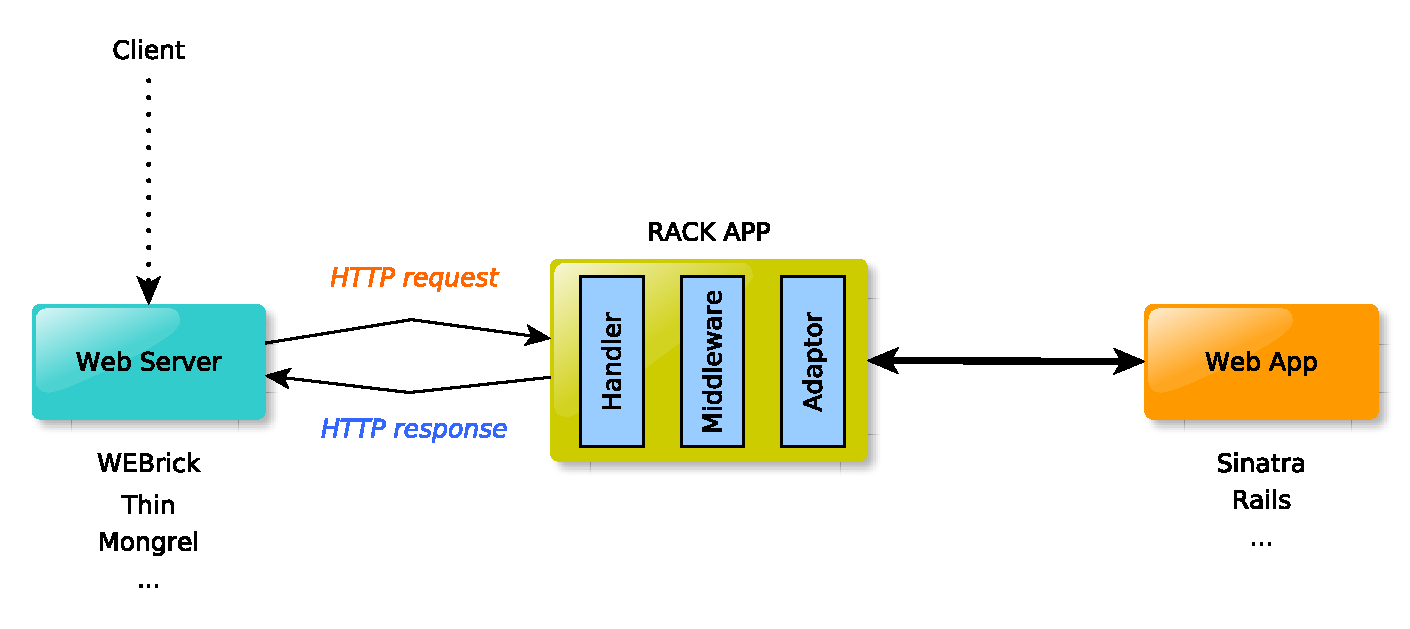
\includegraphics[scale=0.5]{diagrams/rack.pdf}  
  \end{center}

\end{frame}



\begin{frame}[fragile]\frametitle{Rack Example}
  \lstinputlisting[language=ruby]{code/my_rack_app.rb}

  \begin{lstlisting}[language=bash, escapechar={^}]
$ ruby my_rack_app.rb
  \end{lstlisting}
\end{frame}



\begin{frame}\frametitle{Rackup}
  
  \begin{itemize}
  
    \item Tool to run Rack applications
    \item Automatically figures out the environment it is run in
    \begin{itemize}
      \item standalone with WEBrick or Thin, etc. or via FastCGI, CGI
      \item can be used to configure (port, environment, etc.)
    \end{itemize}
    
    \item Typically the web application is written as an independent class
    \item Then, \texttt{rackup} is used to run it    
        
  \end{itemize}

\end{frame}



\begin{frame}[fragile]\frametitle{Rack Example with rackup}
  \lstinputlisting[language=ruby]{code/my_rack_app2.rb}

  \lstinputlisting[language=ruby]{code/rack_config.ru}

  \begin{lstlisting}[language=bash, escapechar={^}]
$ rackup rack_config.rb
  \end{lstlisting}
\end{frame}




\begin{frame}[fragile]\frametitle{Sinatra Example with rackup}
  \lstinputlisting[language=ruby, lastline=9]{code/my_app2.rb}

  \lstinputlisting[language=ruby]{code/rack_sinatra_config.ru}

  \begin{lstlisting}[language=bash, escapechar={^}]
$ rackup rack_sinatra_config.rb
  \end{lstlisting}
\end{frame}





\begin{frame}[fragile]\frametitle{Rackup options}

  \begin{lstlisting}[language=bash, escapechar={^}]
$ rackup -p 8888 rack_sinatra_config.rb
  \end{lstlisting}

  \begin{lstlisting}[language=bash, escapechar={^}]
$ rackup -s thin rack_sinatra_config.rb
  \end{lstlisting}

  \begin{lstlisting}[language=bash, escapechar={^}]
$ rackup -D rack_sinatra_config.rb
  \end{lstlisting}

  \begin{lstlisting}[language=bash, escapechar={^}]
$ rackup -P rack.pid rack_sinatra_config.rb
  \end{lstlisting}

  \begin{lstlisting}[language=bash, escapechar={^}]
$ rackup -E production rack_sinatra_config.rb
  \end{lstlisting}
  
\end{frame}





\subsection{Routes}
\begin{frame}[fragile]\frametitle{Routes}

  \lstinputlisting[language=ruby, firstline=4, lastline=22]{code/routes.rb}

\end{frame}




\begin{frame}[fragile]\frametitle{Testing Routes}

  \begin{itemize}
    \item Using the browser
  \end{itemize}
  
  \begin{lstlisting}[language=bash, escapechar={^}]
http://localhost:4567/hello/Kostas
  \end{lstlisting}

  \begin{itemize}
    \item Using the \texttt{curl}
  \begin{itemize}
    \item tool to transfer data from/to server
    \item many protocols: HTTP, HTTPS, FTP, IMAP, POP, SCP, GOPHER, ...
    \item very powerful: proxy, user athentication, HTTP POST, cookies, ...
  \end{itemize}
  \end{itemize}

  \begin{lstlisting}[language=bash, escapechar={^}]
$ curl http://localhost:4567/hello/Kostas
  \end{lstlisting}

\end{frame}




\begin{frame}[fragile]\frametitle{Testing Routes, cont.}

  \begin{lstlisting}[language=bash, escapechar={^}]
$ curl -v http://localhost:4567/hello/Kostas
  \end{lstlisting}

  \begin{lstlisting}[language=bash, basicstyle=\tiny, escapechar={^}]
* About to connect() to localhost port 4567 (#0)
*   Trying 127.0.0.1... connected
> GET /hello/Kostas HTTP/1.1
> User-Agent: curl/7.22.0 (x86_64-pc-linux-gnu) libcurl/7.22.0 OpenSSL/1.0.1 zlib/1.2.3.4 libidn/1.23 librtmp/2.3
> Host: localhost:4567
> Accept: */*
> 
< HTTP/1.1 200 OK 
< Content-Type: text/html;charset=utf-8
< Content-Length: 12
< X-Xss-Protection: 1; mode=block
< X-Content-Type-Options: nosniff
< X-Frame-Options: SAMEORIGIN
< Server: WEBrick/1.3.1 (Ruby/1.9.3/2012-12-25)
< Date: Sun, 14 Jul 2013 17:17:12 GMT
< Connection: Keep-Alive
< 
* Connection #0 to host localhost left intact
* Closing connection #0
Hello Kostas
  \end{lstlisting}

\end{frame}




\begin{frame}[fragile]\frametitle{Routes, cont.}

  \lstinputlisting[language=ruby, firstline=4, lastline=10]{code/routes2.rb}

  \begin{lstlisting}[language=bash, escapechar={^}]
$ curl http://localhost:4567/hello
Hi stranger!
  \end{lstlisting}
  
  \begin{lstlisting}[language=bash, escapechar={^}]
$ curl -X POST -d "name=Kostas&age=20" http://localhost:4567/hello
Kostas, your age is 20
  \end{lstlisting}
  
\end{frame}




\subsection{Templates}
\begin{frame}[fragile]\frametitle{Hello Form -- HTML}

  \lstinputlisting[language=ruby, firstline=8, lastline=23]{code/routes2.rb}
  
\end{frame}




\begin{frame}[fragile]\frametitle{Hello Form -- HTML, cont.}

  \begin{center}
    \includegraphics[scale=0.5]{images/hello_form.png} 
  \end{center}

  \begin{center}
    \includegraphics[scale=0.6]{images/hello_from_post.png}  
  \end{center}
  
\end{frame}




\begin{frame}[fragile]\frametitle{Hello Form -- HTML, cont.}

  \lstinputlisting[language=ruby, firstline=12, lastline=23]{code/routes2.rb}
  
  \begin{itemize}
    \item Some issues:
    \begin{itemize}
      \item routes provide control logic
      \item HTML provide presentation
      \item Can quickly get out of hand and messy
    \end{itemize}
  \end{itemize}

\end{frame}




\begin{frame}[fragile]\frametitle{Templates Introduction}

  \begin{itemize}
    \item Template Languages
    \begin{itemize}
      \item generate any kind of text from a template
      \item combine plain text with variable substitution and control structures
    \end{itemize}

    \item Common on the Web to generate HTML
    \item A wide variety of templates
    \begin{itemize}
      \item ERB
      \item Haml (HTML abstraction markup language)
    \end{itemize}

  \end{itemize}
\end{frame}


\begin{frame}[fragile]\frametitle{ERB}

  \lstinputlisting[language=ruby]{code/template.erb}
  
  \begin{lstlisting}[language=ruby, escapechar={^}]
$ erb -T 1 template.erb > output.txt
  \end{lstlisting}
  
  \lstinputlisting[language=ruby]{code/erb_render.rb}
  
\end{frame}


\begin{frame}[fragile]\frametitle{Haml}

  \lstinputlisting[language=ruby]{code/template.haml}
  
  \begin{lstlisting}[language=ruby, escapechar={^}]
$ gem install haml
...
Successfully installed haml-4.0.3
$ haml template.haml output.html
  \end{lstlisting}
  
  \lstinputlisting[language=ruby]{code/haml_render.rb}
\end{frame}


\begin{frame}[fragile]\frametitle{Simple HTML form in ERB}

  \lstinputlisting[language=html]{code/proj1/views/form.erb}
  
  \begin{itemize}
    \item Notice, nothing dynamic in this view...
    \item Layout information is not recommended...
  \end{itemize}

\end{frame}




\begin{frame}[fragile]\frametitle{Simple HTML form in Haml}

  \lstinputlisting[language=html]{code/proj1/views/form.haml}
  
  \begin{lstlisting}[language=ruby, escapechar={^}]
$ haml form.haml
  \end{lstlisting}
  
  \begin{itemize}
    \item Notice, nothing dynamic in this view...
    \item Layout information is not recommended...
  \end{itemize}

\end{frame}




\begin{frame}[fragile]\frametitle{Simple HTML form in Haml, cont.}

  \begin{lstlisting}[language=ruby, escapechar={^}]
<html>
  <head>
    <title>Hello Form</title>
  </head>
  <body>
    <h1>Time now is 2013-10-30 17:52:16 +0200</h1>
    <form action='/hello' method='post'>
      <label for='name-id'>Name:</label>
      <input id='name-id' name='name' type='text'>
      <br>
      <label for='age-id'>Age:</label>
      <input id='age-id' name='age' type='text'>
      <br>
      <input type='submit' value='Submit'>
    </form>
  </body>
</html>
  \end{lstlisting}
  
\end{frame}




\begin{frame}[fragile]\frametitle{Tiny Sinatra App: User App}

  \begin{itemize}
    \item Tiny app: store user names and respective ages
  \end{itemize}
  
  \lstinputlisting[language=ruby, basicstyle=\tiny]{code/proj1/user_app.rb}
  
\end{frame}



\begin{frame}[fragile]\frametitle{Tiny Sinatra App: User App, cont.}

  \lstinputlisting[language=ruby]{code/proj1/config.ru}
  
  \begin{itemize}
    \item Using ERB and/or Haml templates
  \end{itemize}
  
  \begin{lstlisting}[language=ruby, escapechar={^}]
$ mkdir views
$ cp form.erb form.haml views/.
  \end{lstlisting}
  
\end{frame}




\begin{frame}[fragile]\frametitle{Tiny Sinatra App: User App, cont. (ERB)}

  \lstinputlisting[language=ruby]{code/proj1/config2.ru}
  
  \lstinputlisting[language=ruby]{code/proj1/user_app2.rb}
  
\end{frame}




\begin{frame}[fragile]\frametitle{Tiny Sinatra App: User App, cont. (Haml)}

  \lstinputlisting[language=ruby]{code/proj1/config3.ru}
  
  \lstinputlisting[language=ruby]{code/proj1/user_app3.rb}
  
\end{frame}



\begin{frame}[fragile]\frametitle{VC -- View-Controller}

  \begin{itemize}
    \item What have we done?
    \begin{itemize}
      \item We separated the view from the routes (controllers)
      \item templates (that represent the view) are in their own files
      \item Cleaner code -- separation of controllers and views
    \end{itemize}
    \item MVC -- Model-View-Controller architecture
    \item Sinatra supports \textit{VC} out of the box

  \end{itemize}

\end{frame}



\subsection{Databases and Models}
\begin{frame}[fragile]\frametitle{Database Frameworks}

  \begin{itemize}
    \item Relational Database
    \begin{itemize}
      \item Postgresql, MySQL, MariaDB, \textbf{Sqlite}
      \item Sqlite (simple and efficient -- for learning and testing)
      \begin{itemize}
        \item Zero configuration
        \item Server-less
        \item Single database file
        \item Stable cross-platform database file
        \item Very fast reads for single user operation
      \end{itemize}

    \end{itemize}

    \item Database Frameworks
    \begin{itemize}
      \item Why: differences between database vendors
      \item What: Abstract the database (SQL and everything...)
      \item How: Implement programming API that translates to SQL and specific database calls
      \item ActiveRecord, \textbf{Sequel}, DataMapper
    \end{itemize}

  \end{itemize}

\end{frame}




\begin{frame}[fragile]\frametitle{Sequel (Just a Ruby API, no SQL)}

  \begin{lstlisting}[language=bash, escapechar={^}]
$ gem install sqlite3 sequel
$ mkdir db
$ touch db/users.db
$ mkdir scripts
$ vim scripts/init_db.rb 
  \end{lstlisting}

  \lstinputlisting[language=ruby]{code/proj1/scripts/init_db.rb}

  \begin{lstlisting}[language=bash, escapechar={^}]
$ ruby ./scripts/init_db.rb
  \end{lstlisting}
  
\end{frame}




\begin{frame}[fragile]\frametitle{Model -- The \textit{M} of MVC}

  \begin{itemize}
  
    \item Object-Relational Mapping (ORM)
    \begin{itemize}
      \item Typically programming using \textit{objects} 
      \item Typically storing data using \textit{relational} tables
      \item ORM \textit{translates} between the two
    \end{itemize}

    \item A model abstracts a \textit{business} entity of the domain

    \item Programmers interact only with models (objects)

  \end{itemize}

\end{frame}




\begin{frame}[fragile]\frametitle{A User model using Sequel}

  \begin{lstlisting}[language=bash, escapechar={^}]
$ mkdir models
$ vim models/users.rb 
  \end{lstlisting}

  \lstinputlisting[language=ruby]{code/proj1/models/users.rb}
  
\end{frame}



\begin{frame}[fragile]\frametitle{Tiny Sinatra App: Reminder}

  \lstinputlisting[language=ruby]{code/proj1/config3.ru}
  
  \lstinputlisting[language=ruby]{code/proj1/user_app3.rb}
  
\end{frame}




\begin{frame}[fragile]\frametitle{Tiny Sinatra App: Storing a User}

  \lstinputlisting[language=ruby, basicstyle=\tiny]{code/proj1/config4.ru}
  
  \lstinputlisting[language=ruby]{code/proj1/user_app4.rb}
  
\end{frame}




\begin{frame}[fragile]\frametitle{Tiny Sinatra App: Checking database}

  \begin{lstlisting}[language=bash, escapechar={^}]
$ sqlite3 db/users.db 
SQLite version 3.7.9 2011-11-01 00:52:41
Enter ".help" for instructions
Enter SQL statements terminated with a ";"
sqlite> select * from users;
1|Kostas|25
sqlite>
  \end{lstlisting}

  \begin{lstlisting}[language=bash, escapechar={^}]
sequel sqlite://db/users.db
Your database is stored in DB...
1.9.3-p362 :001 > users = DB[:users]
 => #<Sequel::SQLite::Dataset: "SELECT * FROM `users`"> 
1.9.3-p362 :002 > users.all
 => [{:id=>1, :name=>"Kostas", :age=>25}] 
1.9.3-p362 :003 >
  \end{lstlisting}
  
\end{frame}




\subsection{Model-View-Controller}
\begin{frame}[fragile]\frametitle{Model-View-Controller (MVC)}

  \begin{columns}[c] 

    \begin{column}{6cm}
      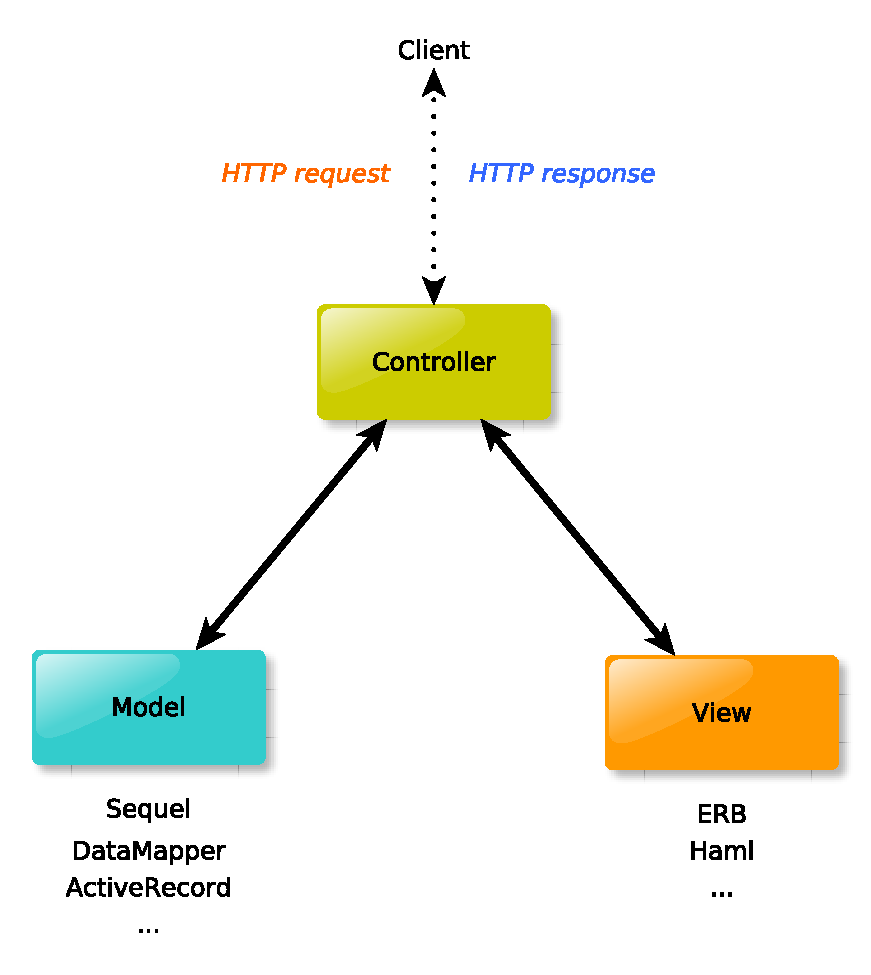
\includegraphics[scale=0.45]{diagrams/mvc.pdf}  
    \end{column}

    \begin{column}{6cm}
      \begin{itemize}
        \item Software Architectural Pattern
        \item Web Development perspective
        \begin{itemize}
          \item Model: represents domain (business) objects
          \item View: output representation of data
          \item Controller: mediates input converting it to commands for the model or view
          \item Note that Model and View have no dependency
        \end{itemize}
        \item Separation of Concerns
        \item Code Re-usability
      \end{itemize}
    \end{column}

  \end{columns}

\end{frame}




\begin{frame}[fragile]\frametitle{Model-View-Controller (MVC), cont.}

  \begin{itemize}
  
    \item MVC is about understanding separation of concerns
    \item Frameworks guide but cannot enforce proper MVC
    \begin{itemize}
      \item A view has available only data that the controller passed to it
      \begin{itemize}
        \item A view never uses database/Model objects directly
      \end{itemize}
      \item A model is completely independent of both controller and view (passive MVC)
      \item The same model can be presented in multiple ways via multiple views
      \item A controller (route) coordinates between model(s) and view(s)
    \end{itemize}

  \end{itemize}

\end{frame}




\subsection{Layout}
\begin{frame}[fragile]\frametitle{Tiny Sinatra App: More Views}
  
  \lstinputlisting[language=ruby]{code/proj1/user_app5.rb}

  \lstinputlisting[language=ruby]{code/proj1/views/hello.haml}
  
\end{frame}




\begin{frame}[fragile]\frametitle{Tiny Sinatra App: More Views, cont.}
  
  \begin{center}
    \includegraphics[scale=.5]{images/hello_form2.png} 
  \end{center}

  \begin{center}
    \includegraphics[scale=.5]{images/hello_from_post2.png}  
  \end{center}  

\end{frame}



\begin{frame}[fragile]\frametitle{Tiny Sinatra App: Adding a Layout}
  
  \lstinputlisting[language=bash]{code/proj1/views/hello.haml}

  \lstinputlisting[language=bash]{code/proj1/views/form.haml}

\end{frame}





\begin{frame}[fragile]\frametitle{Tiny Sinatra App: Adding a Layout, cont.}

  \lstinputlisting[language=bash]{code/proj1/views/layout.haml}
  
  \lstinputlisting[language=bash]{code/proj1/views/hello2.haml}

  \lstinputlisting[language=bash]{code/proj1/views/form2.haml}

\end{frame}




\begin{frame}[fragile]\frametitle{Tiny Sinatra App: Adding a Layout, cont.}

  \lstinputlisting[language=bash]{code/proj1/user_app6.rb}
  
\end{frame}




\subsection{Partials}
\begin{frame}[fragile]\frametitle{Partials}

  \begin{itemize}
    \item Sub-views that can be added to multiple views
    \item Core re-usability
    \item Can complement layouts
  \end{itemize}

  \begin{lstlisting}[language=ruby, escapechar={^}]
= haml :partial
  \end{lstlisting}

  \begin{lstlisting}[language=ruby, escapechar={^}]
<%= erb :partial %>
  \end{lstlisting}
  
\end{frame}





\subsection{Helpers}
\begin{frame}[fragile]\frametitle{Helpers}

  \begin{itemize}
    \item Methods available in routes and views
    \item For calculations and/or HTML generation
  \end{itemize}
  
  \begin{lstlisting}[language=ruby, escapechar={^}]
# ...

helpers do
  def em(text)
    "<em>#{text}</em>"
  end
end

get '/hello' do
  @subject = 'World'
  haml :hello
end

# ...
  \end{lstlisting}

  \begin{lstlisting}[language=bash, escapechar={^}]
# hello.haml
%p= "Hello " + em(@subject)
  \end{lstlisting}
  
\end{frame}




\subsection{Rake}
\begin{frame}[fragile]\frametitle{Rake}

  \begin{itemize}
    \item Build program similar to \textbf{make}
    \item Typically: \texttt{Rakefile}
  \end{itemize}

  \begin{lstlisting}[language=bash, escapechar={^}]
$ gem install rake
  \end{lstlisting}
  
  \begin{lstlisting}[language=ruby, escapechar={^}]
# Rakefile
task :default => [:start]

task :start do
  exec "rackup config.ru"
end
  \end{lstlisting}

  \begin{lstlisting}[language=bash, escapechar={^}]
$ rake
  \end{lstlisting}
  
\end{frame}



\begin{frame}[fragile]\frametitle{Tiny Sinatra App: Automate DB creation}

  \lstinputlisting[language=ruby, basicstyle=\tiny]{code/proj1/Rakefile}

\end{frame}




\begin{frame}[fragile]\frametitle{Tiny Sinatra App: Automate DB creation, cont.}

  \begin{lstlisting}[language=bash, escapechar={^}]
$ rake
[2013-07-24 20:20:02] INFO  WEBrick 1.3.1
[2013-07-24 20:20:02] INFO  ruby 1.9.3 (2012-12-25) [x86_64-linux]
[2013-07-24 20:20:02] INFO  WEBrick::HTTPServer#start: pid=5229 port=9292
  \end{lstlisting}

  \begin{lstlisting}[language=bash, escapechar={^}]
$ rake db
touch db/users.db
/home/karask/.rvm/rubies/ruby-1.9.3-p362/bin/ruby scripts/init_db.rb
Cleaned and initialised db schema
  \end{lstlisting}
  
  \begin{lstlisting}[language=bash, escapechar={^}]
$ rake -D db
rake db:clean
    Deletes the database

rake db:init
    Creates the database schema: db is ready to be populated

  \end{lstlisting}
  
\end{frame}




\subsection{Bundler}
\begin{frame}[fragile]\frametitle{Bundler}

  \begin{itemize}
    \item Managing application dependencies
    \begin{itemize}
      \item Maintaining a consistent environment for ruby applications
      \item Multiple developers and/or multiple machines
    \end{itemize}
    
    \item Specify dependencies: \texttt{Gemfile}
  \end{itemize}
  
  \begin{lstlisting}[language=bash, escapechar={^}]
$ gem install bundler
  \end{lstlisting}
  
\end{frame}



\begin{frame}[fragile]\frametitle{Tiny Sinatra App: Managing Dependencies}

  \lstinputlisting[language=ruby]{code/proj1/Gemfile}

  \begin{lstlisting}[language=bash, escapechar={^}]
$ bundle install
$ git add Gemfile Gemfile.lock
  \end{lstlisting}
  
  \lstinputlisting[language=ruby]{code/proj1/config7.ru}

  \begin{lstlisting}[language=bash, escapechar={^}]
$ bundle exec rackup config7.ru
  \end{lstlisting}
  
\end{frame}




\subsection{Directory Structure}
\begin{frame}[fragile]\frametitle{Directory Structure}

  \begin{center}
    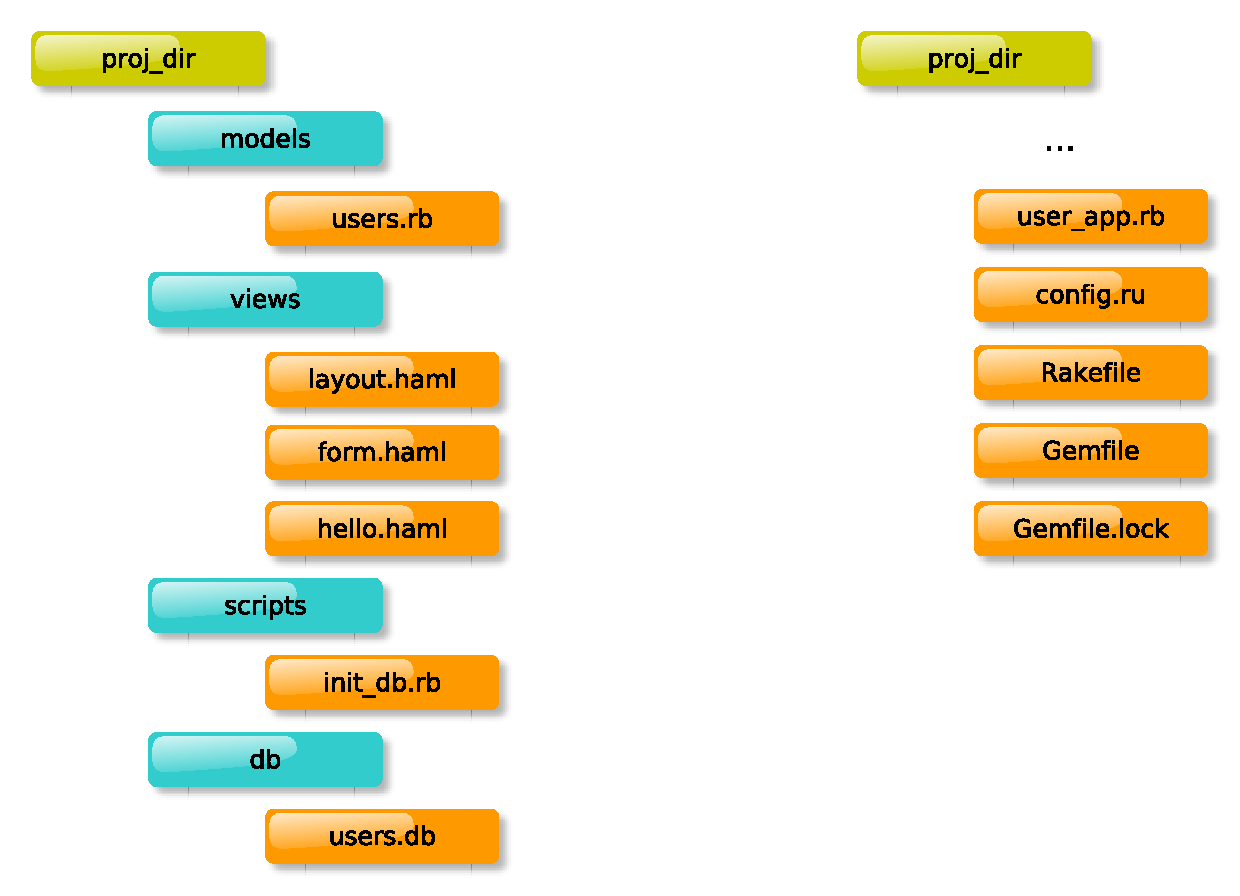
\includegraphics[scale=0.5]{diagrams/dir_structure.pdf}  
  \end{center}
  
\end{frame}



\end{document}
